%_______________________________________________________________________________
%class
%_______________________________________________________________________________
%\documentclass[a4paper,11pt,onecolumn,final,german,openbib]{scrbook}
\documentclass[a4paper,11pt,oneside,final,german,openbib,pdftex]{scrbook}
%_______________________________________________________________________________
% page borders
%_______________________________________________________________________________
\addtolength{\headheight}{2cm}
%\addtolength{\topmargin}{2cm}
\setlength{\oddsidemargin}{1.0cm}
\setlength{\evensidemargin}{0.5cm}
\setlength{\textwidth}{14.3cm}
\setlength{\parindent}{0mm}

%_______________________________________________________________________________
% packages
%_______________________________________________________________________________
\usepackage{german}
\usepackage{amsmath, amssymb}
\usepackage[utf8]{inputenc}
\usepackage{graphicx}
\usepackage{enumerate}
\usepackage{multirow}
\usepackage{subfigure}
\usepackage{dsfont}
\usepackage{slashed}
\usepackage{textcomp}
\usepackage{url}
\usepackage{amsmath}
%_______________________________________________________________________________
% bold fonts for headings
%_______________________________________________________________________________
\font\afont=cmssbx10 scaled \magstep5     % for the title
\font\bfont=cmssbx10 scaled \magstep4     % for chapter headings
\font\cfont=cmssbx10 scaled \magstep3
\font\dfont=cmssbx10 scaled \magstep2     % for section headings and author name
\font\efont=cmssbx10 scaled \magstephalf

%_______________________________________________________________________________
% index depth
%_______________________________________________________________________________
\setcounter{secnumdepth}{3}
\setcounter{tocdepth}{3}

%_______________________________________________________________________________
% new commands
%_______________________________________________________________________________
\newcommand{\demi}{\frac{1}{2}}

%_______________________________________________________________________________
% renewed commands
%_______________________________________________________________________________
% \renewcommand{\topfraction}{1.}       % this is important for figure placement
% \renewcommand{\bottomfraction}{1.}
\makeatletter
\renewcommand\paragraph{\@startsection{paragraph}{4}{\z@}%
  {-3.25ex\@plus -1ex \@minus -.2ex}%
  {1.5ex \@plus .2ex}%
  {\normalfont\normalsize\bfseries}
}
\makeatother

%_______________________________________________________________________________
% special words, hyphenation
%_______________________________________________________________________________
\hyphenation{Ba-che-lor-ar-beit}

\pagestyle{empty}
\pagestyle{headings}
%for changing the style on a specific page use \thispagestyle{e.g., empty}

%_______________________________________________________________________________
%_______________________________________________________________________________
\begin{document}
\pagenumbering{roman}

%_______________________________________________________________________________
\begin{titlepage}
  \vspace*{6mm}
  \begin{center}
     {\afont Titel der Bachelorarbeit}
     \\[3.5cm]
     {\large von}
     \\[3.5cm]
     {\dfont Johanna Musterfrau}
     \\[2cm]
     {\large Bachelorarbeit in Physik \/\\
        vorgelegt dem Fachbereich Physik, Mathematik und Informatik (FB 08) \/\\
        der Johannes Gutenberg-Universit\"at Mainz \/\\
        am 1. April 2012}
   \end{center}
   \vfill
   1. Gutachter: Prof. Dr. Lebeim Elfenbeinturm\\	
   2. Gutachter: Prof. Dr. Habe D\"unkel \\
   \vfill
\end{titlepage}

\thispagestyle{empty}
Ich versichere, dass ich die Arbeit selbstst\"andig verfasst und keine 
anderen als die angegebenen Quellen und Hilfsmittel benutzt sowie 
Zitate kenntlich gemacht habe.
\\
\\[3.5cm] 
Mainz, den [Datum] [Unterschrift]
\vfill
\noindent 
Johanna Musterfrau\\
KOMET\\
Institut f\"ur Physik\\
Staudingerweg 7\\
Johannes Gutenberg-Universit\"at
D-55099 Mainz\\
%{\tt Johanna.Musterfrau@uni-mainz.de}

%_______________________________________________________________________________
\renewcommand\contentsname{Inhaltsverzeichnis}
\renewcommand\figurename{Abbildung}
\renewcommand\tablename{Tabelle}
\tableofcontents
\clearpage

\mainmatter
\sloppy

%_______________________________________________________________________________
\chapter{Einleitung}

{\em Dieses Dokument richtet sich an Studierende am Fachbereich 08 im 
Studiengang Bachelor of Science (Physik). Sie finden hier Beispiele 
f\"ur eine m\"ogliche Gliederung Ihrer Arbeit und Hinweise zur 
Strukturierung des Inhalts. Selbstverst\"andlich sollen Sie diese 
Gliederung nach den Gegebenheiten Ihrer Bachelorarbeit anpassen. 
Besprechen Sie rechtzeitig mit Ihrem Betreuer, ob Ihr Entwurf sinnvoll 
ist. Holen Sie sich auch Anregungen zur Gestaltung von Abschlussarbeiten 
aus der Literatur (siehe z.\ B.\ \cite{EbelBliefert}).
\medskip

Sofern Sie sich dazu entscheiden, Ihr Dokument in \LaTeX\ zu erstellen, 
k\"onnen Sie diese Datei als Vorlage verwenden. Fast die gesamte 
Literatur in der Physik verwendet \LaTeX, vor allem wegen der 
ausgezeichneten M\"oglichkeiten f\"ur das Formelschreiben.
}
\bigskip

In der Einleitung Ihrer Bachelorarbeit sollte das Thema der Arbeit 
m\"oglichst allgemeinverst\"andlich eingef\"uhrt werden. Gehen Sie 
dabei auch auf das weitere Umfeld der Arbeit ein und erl\"autern Sie, 
warum Aufgabenstellung und Herangehensweise interessant sind. Auch 
die weitere Gliederung kann angesprochen werden, um dem Leser einen 
ersten \"Uberblick \"uber den nachfolgenden Text zu geben.

%_______________________________________________________________________________
\chapter{Experimental Setup at SuperKEKB}

SuperKEKB is an electron positron accelerator, which is located at KEK (\textit{High Energy Accelerator Research Organisation}) in Tsukuba Japan. The two beams have an asymmetric energy. 
The electron beam has an energy of $7\ \textnormal{GeV}$ 
and the positron beam have an energy of $4\ \textnormal{GeV}$. These beams collide with a center-of-momentum energy of about $10.58\ \textnormal{GeV}$, which is close to the mass of the $\Upsilon(4\textnormal{S})$ resonance. Therefore SuperKEKB is a so called \textit{B-factory}. The decay products are then detected by the  Belle II detector to study the properties of these B mesons with high precision. In early 2018 Belle II started taking data. One goal of Belle II is to study CP-Violation with respect to new physics.

\section[KEK]{KEKB and SuperKEKB}






%Die typische Gliederung einer Bachelorarbeit k\"onnte so aussehen, 
%wie im folgenden dargestellt. 
\medskip

%Verwenden Sie aussagekr\"aftige Kapitel\"uberschriften, also zum 
Beispiel {\em Aufbau eines Teilchenbeschleunigers} statt 
{\em Versuchsaufbau}.


%_______________________________________________________________________________
\section{Grundlagen}

Beschreiben Sie bei einer experimentellen Arbeit die wesentlichen 
theoretischen Grundlagen und in jedem Fall den Stand der Forschung.

\section{Versuchsaufbau}

Wenn Sie an einem experimentellen Thema arbeiten, beschreiben Sie 
den Versuchsaufbau, auch wenn Sie an einem bereits vorhandenen 
Versuch arbeiten, soweit dies f\"ur Ihre spezielle Fragestellung 
relevant ist. 

\section{Methoden}

Entsprechend kann es bei einer theoretischen Arbeit sinnvoll sein,
die L\"osungsmethoden in einem eigenen Kapitel zu beschreiben.

\section{Ergebnisse}

Hauptteil Ihrer Arbeit ist das Kapitel (oder die Kapitel) mit den 
Ergebnissen. Bei einer theoretischen Arbeit kann damit auch 
die Herleitung von Formeln oder die Beschreibung eines Computerprogramms 
gemeint sein.

%_______________________________________________________________________________
\chapter{Zusammenfassung und Ausblick}

In der Zusammenfassung sollten Sie in knapper Form die Aufgabenstellung 
und die wichtigsten Ergebnisse rekapitulieren. Es ist f\"ur die 
Gutachter hilfreich, wenn Sie ausdr\"ucklich beschreiben, worin 
Ihre eigenen Beitr\"age liegen. Scheuen Sie sich auch nicht davor 
auszusprechen, welche Untersuchungen durch die Zeitbegrenzung der 
Bachelorarbeit nicht m\"oglich waren und nutzen Sie dies als 
\"Uberleitung zu einem Ausblick auf m\"ogliche weitergehende 
Arbeiten an der Aufgabenstellung.

%_______________________________________________________________________________
\begin{appendix}
\chapter{Anhang}

\section{Tabellen und Abbildungen}

In der Regel sind die in Tabellen und Abbildungen enthalten Informationen 
so wichtig, dass sie im Hauptteil der Arbeit erscheinen sollten. Unter 
Umst\"anden sind aber erg\"anzende Tabellen und Abbildungen gut in einem 
Anhang aufgehoben. Wie im Hauptteil sollten Sie auch hier darauf achten, 
dass die in Tabellen und Figuren (siehe Abb.\ \ref{Abb:1}) dargestellte 
Information im Text angesprochen wird und selbsterkl\"arende Legenden 
vorhanden sind.
\medskip

\begin{figure}[h]
\begin{center}
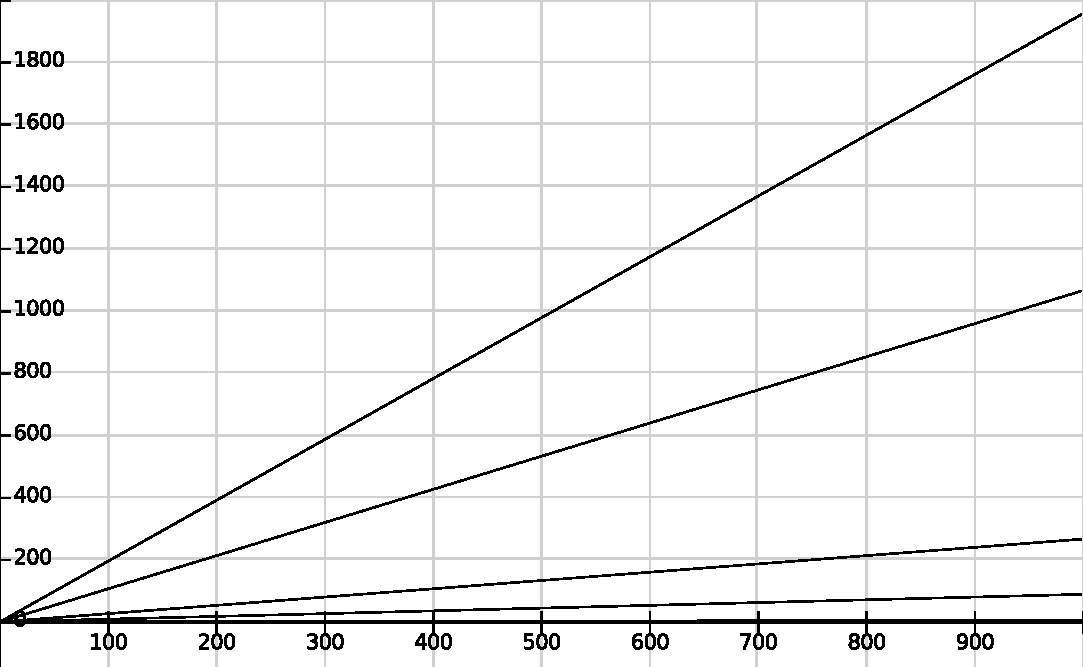
\includegraphics[scale=0.8]{BA-Abbildung1.pdf}
\end{center}
\caption{\label{Abb:1}
Feynmandiagramm f\"ur eine typische Einschleifen-Korrektur zur 
Produktion von sieben Jets in der $e^+e^-$-Vernichtung (entnommen 
aus \cite{thepnews}, mit Zustimmung der Autoren).
} 
\end{figure}


%_______________________________________________________________________________
\section{Weiterf\"uhrende Details zur Arbeit}

Manch wichtiger Teil Ihrer tats\"achlichen Arbeit ist zu technisch 
und w\"urde den Hauptteil des Textes un\"ubersichtlich machen, 
beispielsweise wenn es um die Details des Versuchsaufbaus in einer 
experimentellen Arbeit oder um den f\"ur eine numerische Auswertung 
verwendeten Algorithmus geht. Dennoch ist es sinnvoll, entsprechende 
Beschreibungen in einem Anhang Ihrer Bachelorarbeit aufzunehmen. 
Insbesondere f\"ur zuk\"unftige Arbeiten, die an Ihre Bachelorarbeit 
anschlie{\ss}en, sind dies manchmal hilfreiche Informationen.

%_______________________________________________________________________________
\chapter{Literaturverzeichnis}

Machen Sie genaue Angaben, so dass die verwendeten Literaturstellen 
eindeutig identifiziert und aufgefunden werden k\"onnen.
Bei Lehrb\"uchern \cite{Weinberg:1995mt} ist es sinnvoll, 
den Titel anzugeben, eventuell auch die Ausgabe. Bei Artikeln in 
Fachzeitschriften \cite{Moch:2001zr} ist es \"ublich, nur die 
gebr\"auchlichen Abk\"urzungen f\"ur den Titel der Zeitschrift, Band, 
Erscheinungsjahr und Seite anzugeben. Unter Umst\"anden kann es auch 
sinnvoll sein, im Internet aufgefundene Informationsquellen anzugeben, 
zum Beispiel f\"ur Software \cite{LoopTools} oder zu den Details von 
Ergebnissen gro{\ss}er experimenteller Kollaborationen. Es ist 
selbstverst\"andlich, dass Sie auch Bachelor- \cite{BA:Freund}, 
Diplom- oder Doktorarbeiten angeben, wenn Sie diese in Ihrer eigenen 
Arbeit verwendet haben.
\medskip

Im folgenden Beispiel werden die in der Datei %{\tt h-physrev3.bst} 
enthaltenen Anweisungen als Stilvorlage verwendet. Andere 
M\"oglichkeiten f\"ur die Gestaltung eines Literaturverzeichnisses 
findet man im Internet: \url{http://janeden.net/bibliographien-mit-latex}.

\renewcommand{\bibname}{\bfont Literaturverzeichnis} 
\bibliographystyle{h-physrev3}
\begin{thebibliography}{99}

%\cite{thepnews}
\bibitem{EbelBliefert}
H.\ F.\ Ebel, C.\ Bliefert, 
  ``Bachelor-, Master- und Doktorarbeit: Anleitungen f\"ur den 
  naturwissenschaftlich-technischen Nachwuchs,''
  Wiley-VCH, Weinheim (2009). 
\bibitem{thepnews}
  S.~Becker, D.~G\"otz, C.~Reuschle, C.~Schwan, S.~Weinzierl,  
  \url{http://wwwthep.physik.uni-mainz.de/site/news/168/}.

%\cite{Weinberg:1995mt}
\bibitem{Weinberg:1995mt}
  S.~Weinberg,
  ``The Quantum theory of fields. Vol. 1: Foundations,''
  Cambridge, UK: Univ. Pr. (1995) 609 p.

%\cite{Moch:2001zr}
\bibitem{Moch:2001zr}
  S.~Moch, P.~Uwer, S.~Weinzierl,
  %``Nested sums, expansion of transcendental functions and multiscale 
  % multiloop integrals,''
%  J.\ Math.\ Phys.\  {\bf 43 } (2002)  3363-3386.
  [hep-ph/0110083].

%\cite{LoopTools}
\bibitem{LoopTools}
  T.~Hahn, 
  ``The LoopTools Site,''
  \url{http://www.feynarts.de/looptools/}.

%\cite{BA:Freund}
\bibitem{BA:Freund}
  B.~Freund, 
  Bachelorarbeit, Johannes Gutenberg-Universit\"at Mainz, 2012.

\end{thebibliography}

%_______________________________________________________________________________
\chapter{Danksagung}

... an wen auch immer. Denken Sie an Ihre Freundinnen und Freunde, 
Familie, Lehrer, Berater und Kollegen.

\end{appendix}

\end{document}  
        
        